\chapter {Experiment}

\section{Non-Catalysed Experiment Series}

In order to work out the order of sulfuric acid in the Zinc and sulfuric acid reaction I carried out an experiment without the presence catalyst. I varied the concentration of the sulfuric acid (6 series with a range of 2.0 Molar - 6.0 Molar) whilst keeping the mass of Zinc the same (1.0 g). My raw data tables can be seen below for each concentration of sulfuric acid.

	\subsection{2.0 Molar Sulfuric Acid}

\begin{figure}[H]
    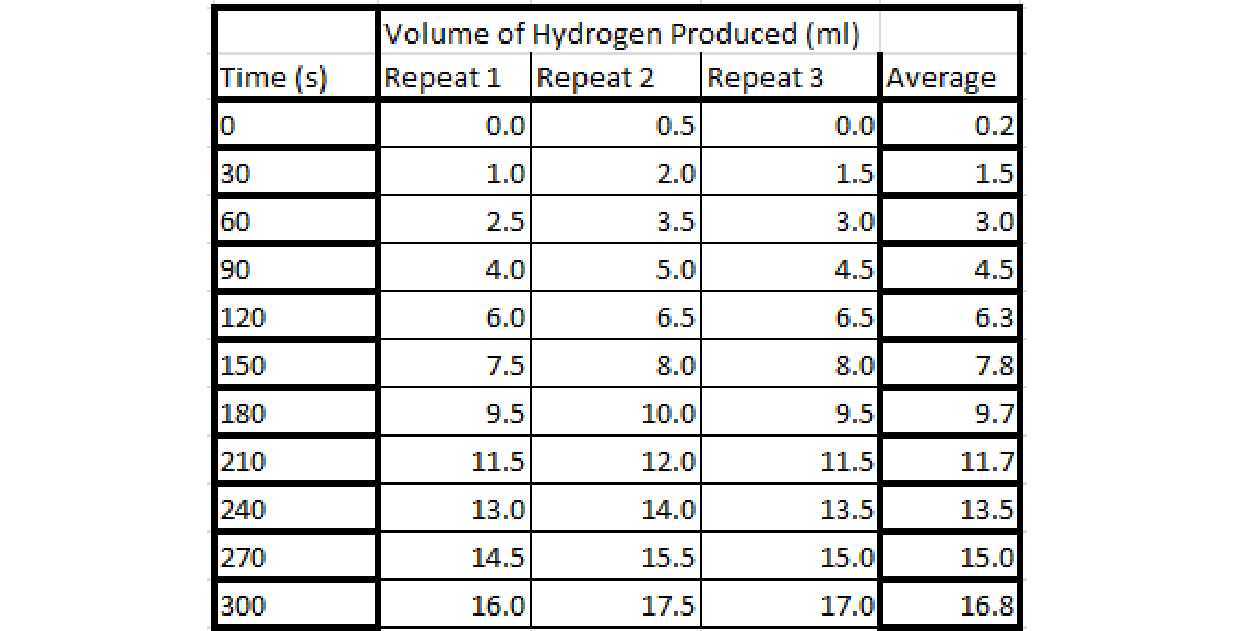
\includegraphics[width=\textwidth]{./Experiment/Images/1NonCatalyst/2Molar.pdf}
    \caption{ Rate vs Concentration First-Order Graph} \label{fig:First Order Graph}
\end{figure}


	\subsection{2.4 Molar Sulfuric Acid}

	\subsection{2.8 Molar Sulfuric Acid}

	\subsection{3.2 Molar Sulfuric Acid}

	\subsection{3.6 Molar Sulfuric Acid}

	\subsection{4.0 Molar Sulfuric Acid}

\section{Copper Sulfate Catalysed Experiment Series}

EXPLAIN EXPERIMENT - Acid may be a different order in presence of a catalyst. 0.01molar Copper sulfate 

	\subsection{0.2 Molar Sulfuric Acid}

	\subsection{0.4 Molar Sulfuric Acid}

	\subsection{0.6 Molar Sulfuric Acid}

	\subsection{0.8 Molar Sulfuric Acid}

	\subsection{1.0 Molar Sulfuric Acid}

	\subsection{1.2 Molar Sulfuric Acid}


\section{Varying Copper Sulfate Experiment Series}

EXPLAIN EXPERIMENT - To find the order of copper sulfate in the reaction.

	\subsection{0.01 Molar Copper Sulfate}

	\subsection{0.02 Molar Copper Sulfate}

	\subsection{0.03 Molar Copper Sulfate}

	\subsection{0.04 Molar Copper Sulfate}

	\subsection{0.05 Molar Copper Sulfate}

	\subsection{0.06 Molar Copper Sulfate}



\section{Different Catalysts Experiment Series}

After finishing my initial experiment, I began to think about how different catalysts affect the rate of reaction. 


\section{Solubility of Hydrogen Experiment Series}

As shown by my BLAH. 